\chapter{Project Definition}
\section{Definition Revisions}
The definition has been reviewed and the scope was deemed too large.
It was then decided that the project would be redefined as a CNC Interface.

The CNC Interface will be the interface to interpret G-code and to the motor driver board.
The revised product will be configurable to operate on different mechanical systems. 
The current system for converting G-code for use on a CNC currently requires a whole computer. 
With this system, a web interface will be utilized to upload the G-code files.
A master controller will be used to interpret this G-code to motor commands. 
These commands will be sent to the motor driver board that will drive the motors.
Making this interface automated will improve the ability for students and hobbyists to have their own CNC Interface for 3D printing or PCB milling.

\subsection{Revised Objective Tree}

\begin{figure}[H]
\centering
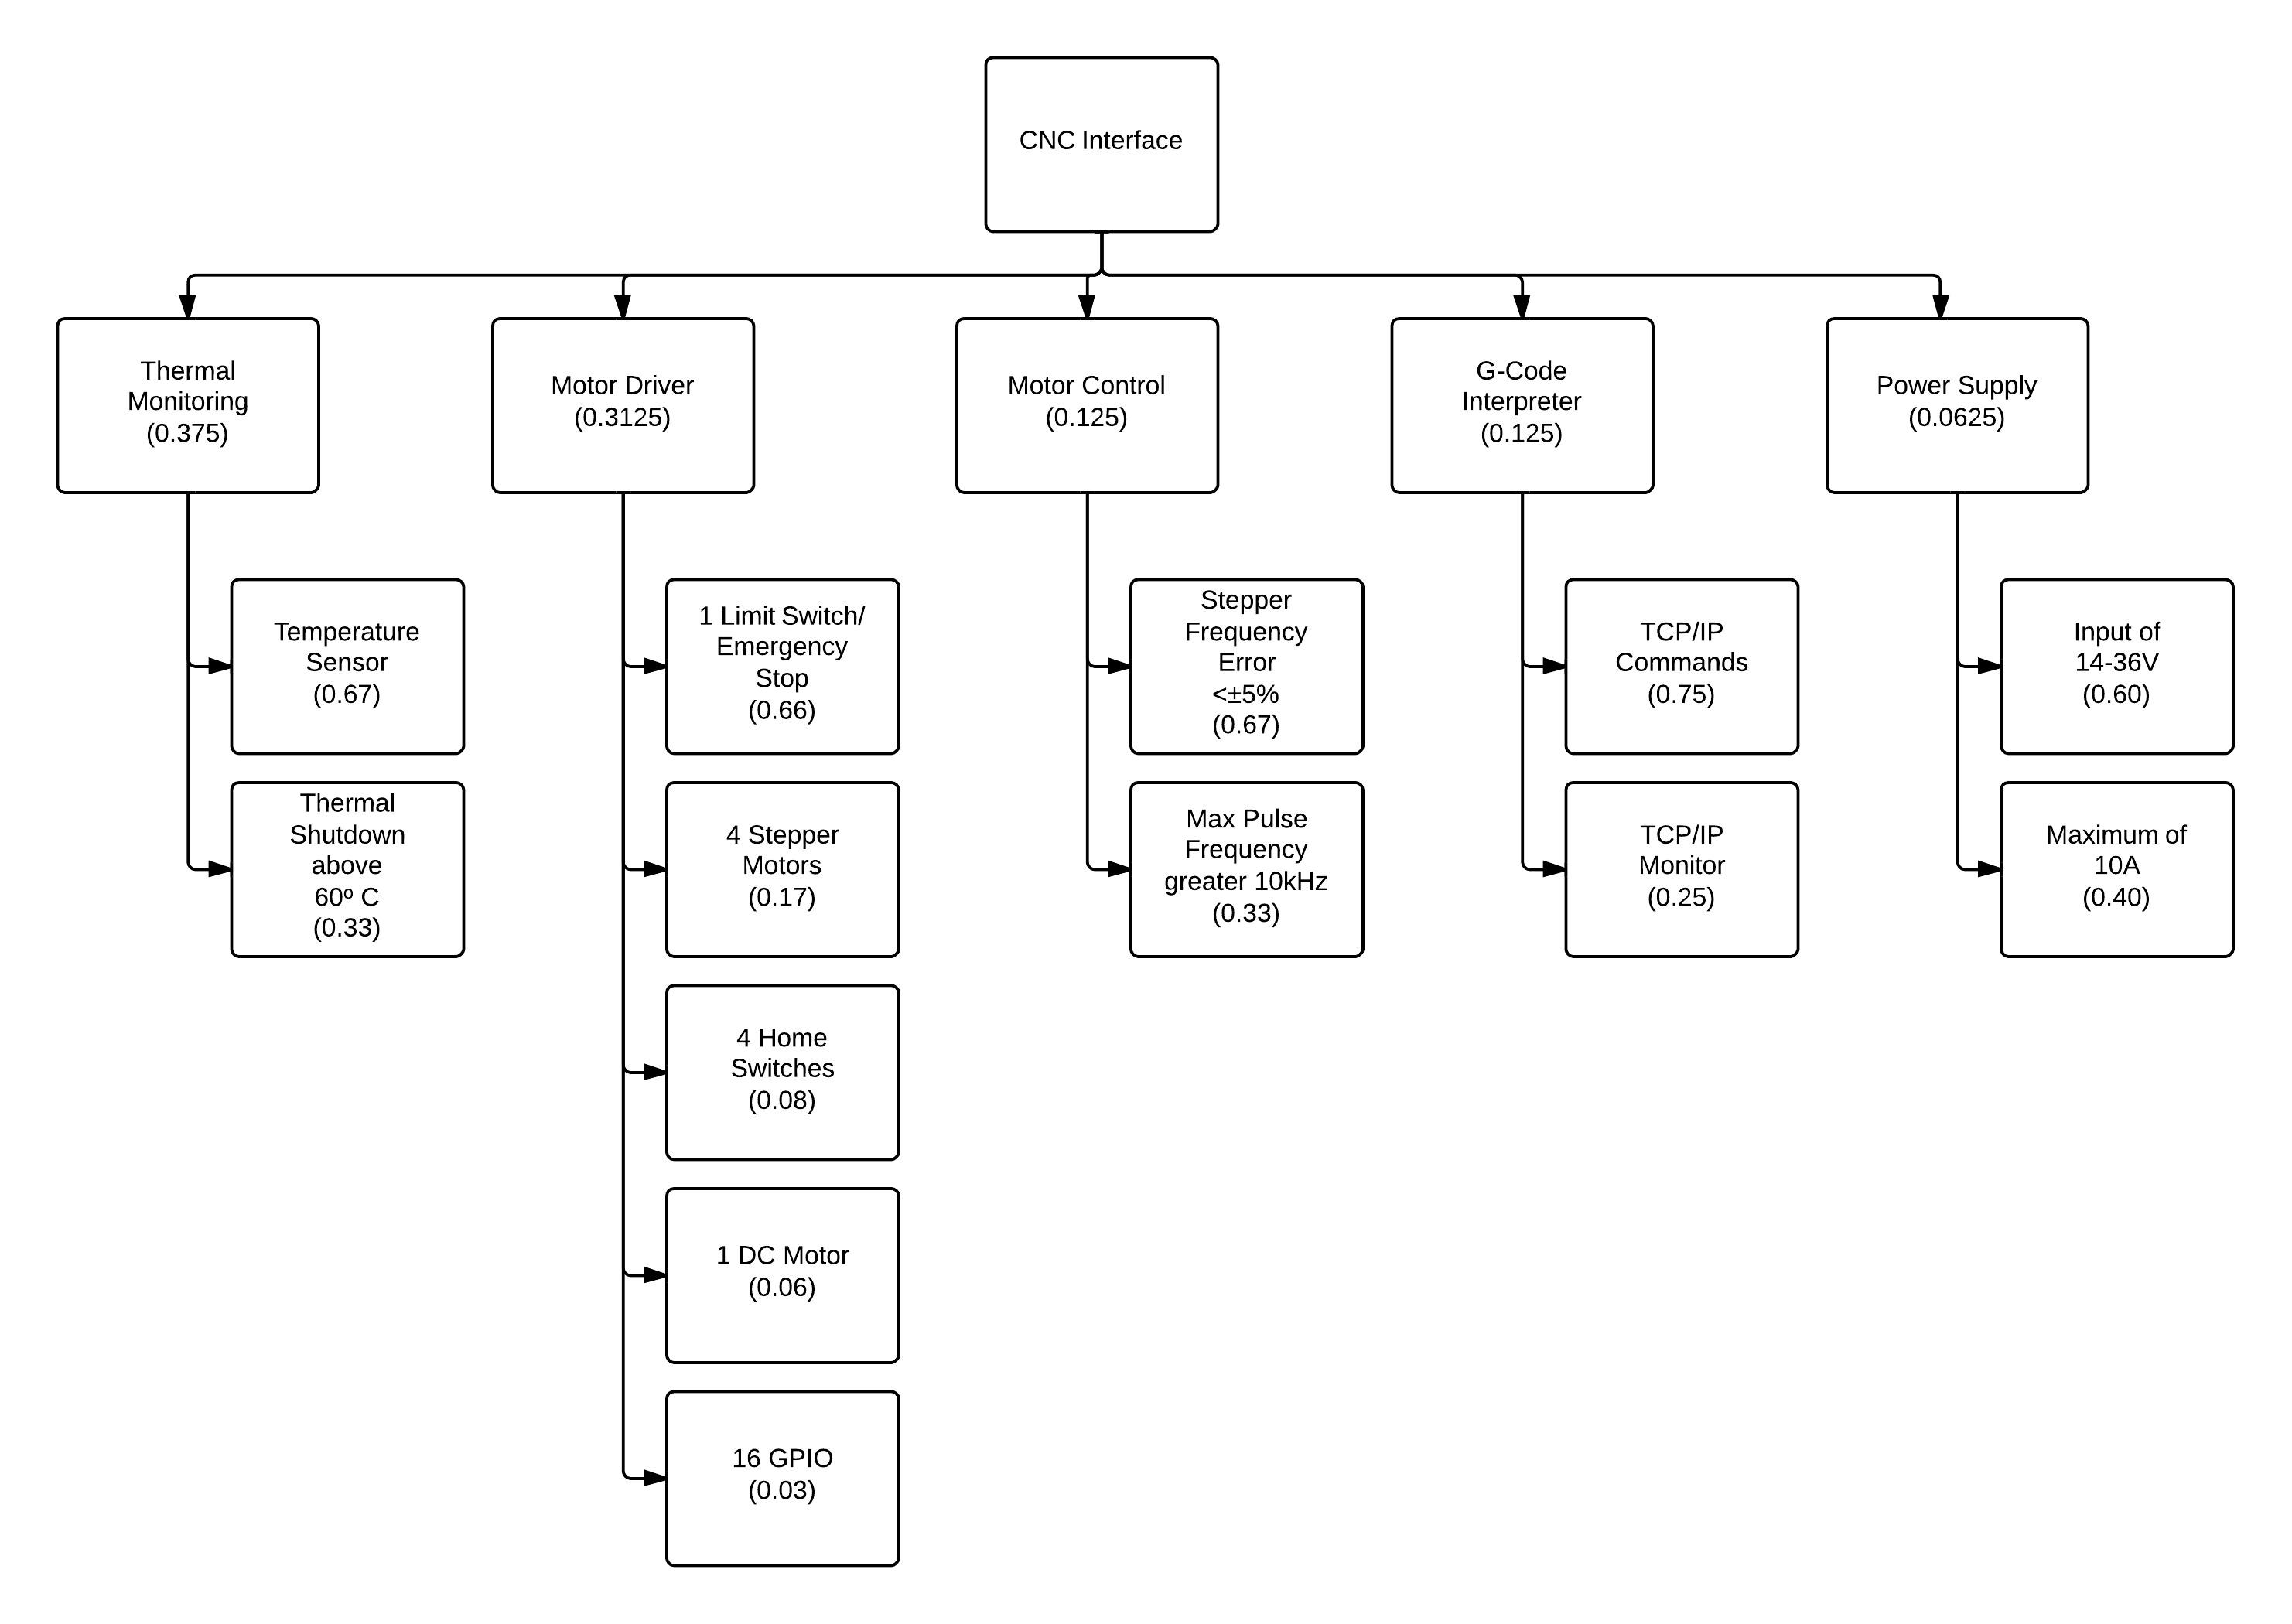
\includegraphics[width=1.0\textwidth]{otree.jpeg}
\caption{Stakeholder Chart}
\label{fig:Stakeholder Chart}
\end{figure}

The objective tree has been revised to reflect objectives that are verifiable.
Thermal Monitoring was weighted as most important because it is a safety feature.
The Motor Driver is a second priority because it is the main functionality.
The Motor Control and G-Code Interpreter were decided to be equally important by using Piecewise Comparisons.
Motor Control relates to the motor accuracy.
G-Code Interpretation is the software interface that will allow a file to be uploaded and sent through TCP/IP.
The Power Supply is least important because it can be easily standardized and not left up to the user.
\subsection{Revised Statement of Project Scope}
The Project Scope has been refocused. 
The mechanical requirements and the human-machine interfacing for the project have been eliminated.
The scope now only includes the software for the G-code interpretation, its upload interface, the master controller, the motor controller and the motor driver board.
The G-code interpretation software will have a G-code file as an input and then output motor driver commands from the master controller to the motor controller.
The motor controller will then send out the driver signals to the motor driver board. 
The motor driver board will take the command outputs from the motor controller and then drive the motors. 
There will also be 16 GPIO pins, an emergency stop switch, and home switches for the motors. 
With this redefined scope, a more polished end product will be achieved. 
\section{Microprocessor Functionality}
The main microprocessor, an \gls{arm} 11 on the \gls{pi}, will primarily be responsible for controlling the three stepper motors for the delta robot.
This objective will be achieved by creating a G-code interpreter written in C.
G-code is a standard way to instruct a \gls{cnc} router to move the work head, but is more complicated than accepting individual commands to move the motors.
The microprocessor will be responsible for scheduling movements to make smooth transitions to the destination, as interpreted from the G-code.

The system will mainly be a network device, connected through WiFi or Ethernet.
The microprocessor will obtain G-code commands through local storage or by accepting G-code files over TCP/IP.
The G-code received over TCP/IP and will be stored locally for faster use again in the future.
Execution of G-code sequences will be started through a TCP/IP interface.
All network interfaces will be password protected and use encryption algorithms to ensure that all commands executed are from authorized users. 

A secondary microprocessor may be required to precisely control stepper motors and the \gls{gpio}.
This secondary microprocessor will perform any required communication with the network-connected main microprocessor through a serial interface. 

\section{CEEN Appropriateness}
The design and execution of the CNC Interface will meet at least 7 of the 11 ABET accreditation criteria.
The design and construction will require the rigorous application of mathematics, science, and engineering for the software, hardware, mechanical, and system control. (ABET 3a).
Notably, the kinematics of the robot will require intense mathematical computations to ensure accuracy.
Experiments must be designed and conducted to ensure proper operation of components and the final result (ABET 3b).
The end result of the project will meet the needs outlined in the Background Summary (ABET 3c).
The level of success of the project will depend on how well the the team is able to cooperate and strive to achieve common goals (ABET 3d).
This project will present many engineering problems that will have to be solved (ABET 3e).
Not only must the group work towards common goals, but they must also communicate effectively (ABET 3g).
Similarly to ABET 3a, the entire project will involve the use of engineering skills that have been learned in previous coursework (ABET 3k).

The senior capstone project also serves as a culmination of the CEEN curriculum. Concepts and skills learned in previous courses must be applied in the design, construction, and documentation of the project.
Courses that will be built upon in the design of the CNC Inteface are:
\begin{enumerate} \parskip2pt
	\item Microprocessor Applications
	\item Electrical \& Electronic Circuits
	\item Communication Systems
	\item Signals \& Linear Systems
	\item Digital Design \& Interface
	\item Microprocessor System Design
	\item Embedded Microcontroller Design
\end{enumerate}

\subsection{Revised Project Charter}
The purpose of this project is to create a final working system that exceeds the expectations of all stakeholders. This goal will be achieved through proper planning and execution with a focus on system testing throughout the process.

\subsection{Roles and Authority}
The following definitions will serve as the guidelines for each team member's major tasks throughout the project lifetime. All team members are expected to help one another out to ensure the best outcomes for the project, not just for the individual's task completion
\paragraph{Faculty Sponsor: Herbert Detloff}
Demonstrates previous experience with several successful capstone design projects.
Provides feedback and assessment of project definition, plan, and status.
Ensures that all team members are aware of the engineering impact of the project on the University of Nebraska - Lincoln and the rest of the world.
Teaches standard engineering principals for project management, development, execution, and testing to aid in the project's completion.

\paragraph{Resource Manager: James Gehringer}
Responsible for promoting collaboration, communicating progress with the faculty sponsor, and procuring resources.
Accountable for intellectual property management in solidification of ideas and iterative verification of project objectives.
Involved with all phases of design in order to better assure both long and short term goals are met with efficiency by keeping track of the progress of the project by setting deadlines, scheduling tasks, and monitoring progress through tools such as Gantt charts.
Oversees documentation and monitors project health to identify issues as soon as possible.

Reports to the Faculty Sponsor. 

\paragraph{Systems Engineer: Evan Milton}
In charge of generating the system's requirements and specifications and understanding the project as a whole, including mechanical, electronic, and software components and their interfacing.
Works closely with the Hardware and Software Development Engineers to best meet the team objectives, system's requirements, and specifications.
Responsible for acceptance testing the prototypes and final project to ensure quality and confirm that all specifications are met.
Determines alternate solutions case any solution fails or becomes unfeasible during development.
Makes final design decisions when challenges arise that require major modifications.

Reports to the Resource Manager and Faculty Sponsor.

\paragraph{Hardware Development Engineer: Chad Staley}
Accountable for developing the design, layout, construction, and testing of the electrical systems required for this project to create a solid platform for the software.
Focused on simplicity and robustness in design, to aid troubleshooting when software is added to the project.
Understands and can communicate the software interfacing that must occur to make the hardware function properly.

Reports to the Systems Engineer, Resource Manager, and Faculty Sponsor. 

\paragraph{Software Development Engineer: Josh Dewitt}
Responsible for the higher level functionality of the project by writing clean, modular code that can be adapted where hardware changes might be cost-prohibitive.
Will communicate with the Hardware Development Engineer to understand the hardware interfacing to meet the requirements set by the Systems Engineer.
Performs domain, software element, and requirements analysis to ensure the code produced matches the needs of the users, then develops code in any language necessary, using test­-driven development.

Reports to the Systems Engineer, Resource Manager, and Faculty Sponsor.

\subsection{Quality Objectives}
The team agrees that output of this capstone design sequence will be high-quality product that is reproducible, robust, and goes beyond expectations.
This objective will be achieved by setting engineering requirements that will use all of our talent, while still being achievable given the time frame of the course, and meeting these set requirements through a team effort.
Rapid prototyping will allow issues to be revealed early in the project's execution, making sure that the correct priorities are set to focus on those items that may cause an engineering requirement to not be met.

\subsection{Revised Requirements Specification}
\textbf{Marketing Requirements}

The system will meet the following criteria:
\begin{enumerate} \parskip2pt
	
	\item be accurate in its motor control.
	\item be quickly accelerate the motors.
	\item be able to send command files through a web interface.
	\item be able to drive multiple motors.
	\item be able to handle general purpose input and output.
	\item be able to be stopped in an emergency.
	\item be able to shutdown if the system gets too hot. 
	\item be able to operate at a range of input voltages.
\end{enumerate}